\documentclass[10pt]{beamer}

\usepackage{gensymb}
\usepackage{graphicx}
\usepackage{wrapfig}
\usepackage{attrib}
\usepackage{textpos}

\usetheme{Dresden}
\usecolortheme{dove}
\usenavigationsymbolstemplate{}
\title{Comparison of Associative Data Structures}
\author{Pieter Brederode, Jelco Bodewes, \\ Timo Koppenberg, Anton Golov}
\institute{B3OMI}


\begin{document}

\begin{frame}
    \maketitle
\end{frame}


\section{Introduction}
\begin{frame}{Overview}
    \begin{itemize}
        \item Problem Statement
        \item Measurement Implementation
        \item Results
        \item Conclusions
    \end{itemize}
\end{frame}

\begin{frame}{Context: Whitelist/Blacklist}
    \begin{itemize}
        \item Program that given a URL decides whether to allow access.
        \item Different possible granualities:
        \begin{itemize}
            \item IP address (32 bit integer)
            \item Domain name (20 char string)
            \item Full path (100 char string)
        \end{itemize}
        \item Fast insert and query
        \item Low memory usage
    \end{itemize}
\end{frame}

\section{Implementation}
\begin{frame}{Implementation}
    \begin{itemize}
        \item C++
        \begin{itemize}
            \item We hoped for predictable performance\ldots
            \item Standard library has hash table and binary search tree
            \item Standard library has timing tools
        \end{itemize}
        \item Open source SkipList library (\texttt{CSSkipList})
        \begin{itemize}
            \item Weird results can be investigated directly
            \item Turned out useful
        \end{itemize}
        \item POSIX API for memory usage
    \end{itemize}
\end{frame}

\begin{frame}{Implementation Issues}
    \begin{itemize}
        \item POSIX API for memory is too coarse
        \begin{itemize}
            \item Added tracking of alloctions
            \item Bonus: only track the data structure itself
            \item Required modifying the SkipList
        \end{itemize}
        \item Performance is consistent, but unusual
        \begin{itemize}
            \item Hash tables are quirky
            \item Suspect: the allocator
            \item Run tests in separate process
            \begin{itemize}
                \item Or write your own allocator\ldots
            \end{itemize}
        \end{itemize}
    \end{itemize}
\end{frame}

\begin{frame}{Small hash tables are expensive}
    \centering
    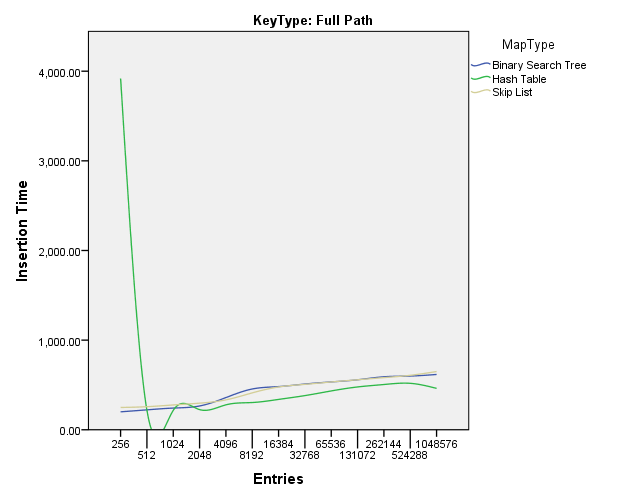
\includegraphics[width=\textwidth]{hashtable_bad.png}
\end{frame}

\begin{frame}{Big hash tables are cheap}
    \centering
    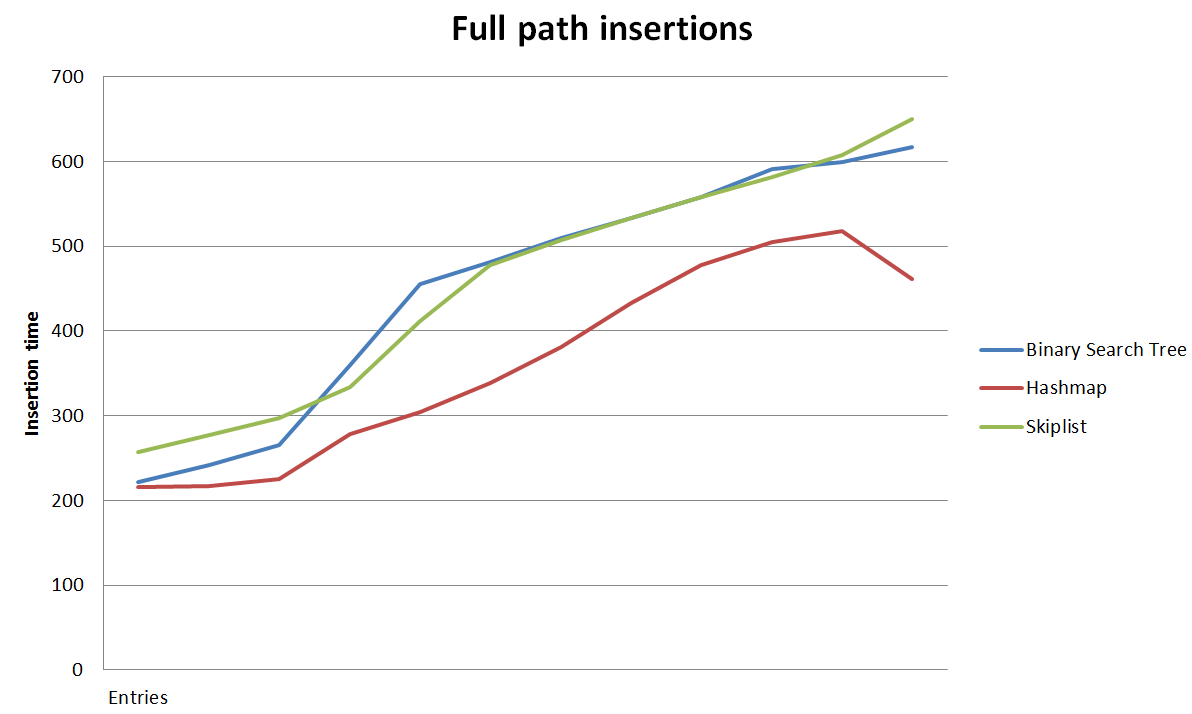
\includegraphics[width=\textwidth]{hashtable_good.png}
\end{frame}

\section{Results}

\begin{frame}{Results}
    \begin{itemize}
        \item 117 different setups.
        \item 19 runs, for a total of 2223 cases.
    \end{itemize}
\end{frame}

\begin{frame}{Number of entries}
    \begin{figure}
      \centering
        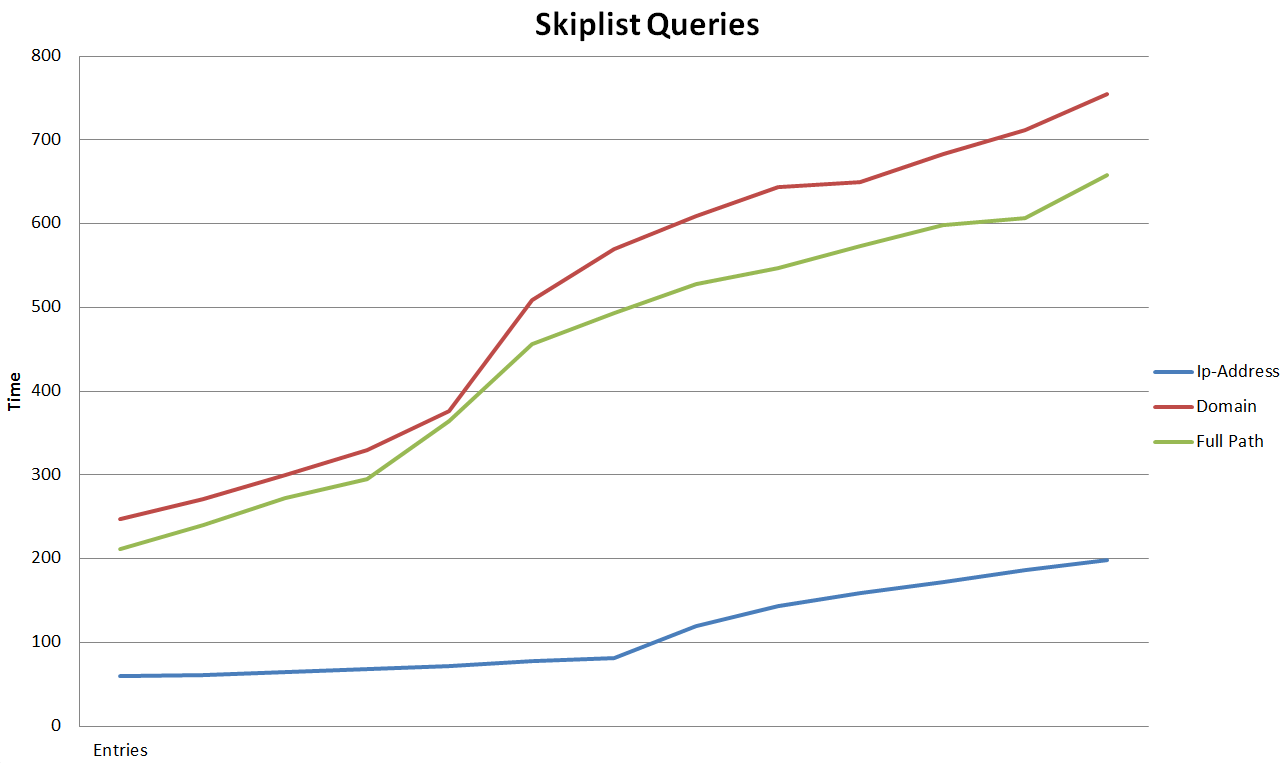
\includegraphics[width=0.95\textwidth]{SkiplistQuery}
      \caption{The average duration of each query operation, plotted against the total number of entries.}
    \end{figure}
\end{frame}

\begin{frame}{Number of entries}
    \begin{itemize}
        \item There is a positive correlation between the number of entries and the average duration of all operations.
        \item This is true for both insert and query average duration.
        \item Not always true for average memory usage.
    \end{itemize}
\end{frame}

\begin{frame}{Number of entries}
    \begin{itemize}
        \item Average memory usage for BST is constant.
        \item Average memory usage for hash table has a positive correlation with the number of entries.
        \item Average memory usage for Skiplist has a negative correlation with the number of entries.
    \end{itemize}
\end{frame}

\begin{frame}{Number of entries}
    \begin{figure}
      \centering
        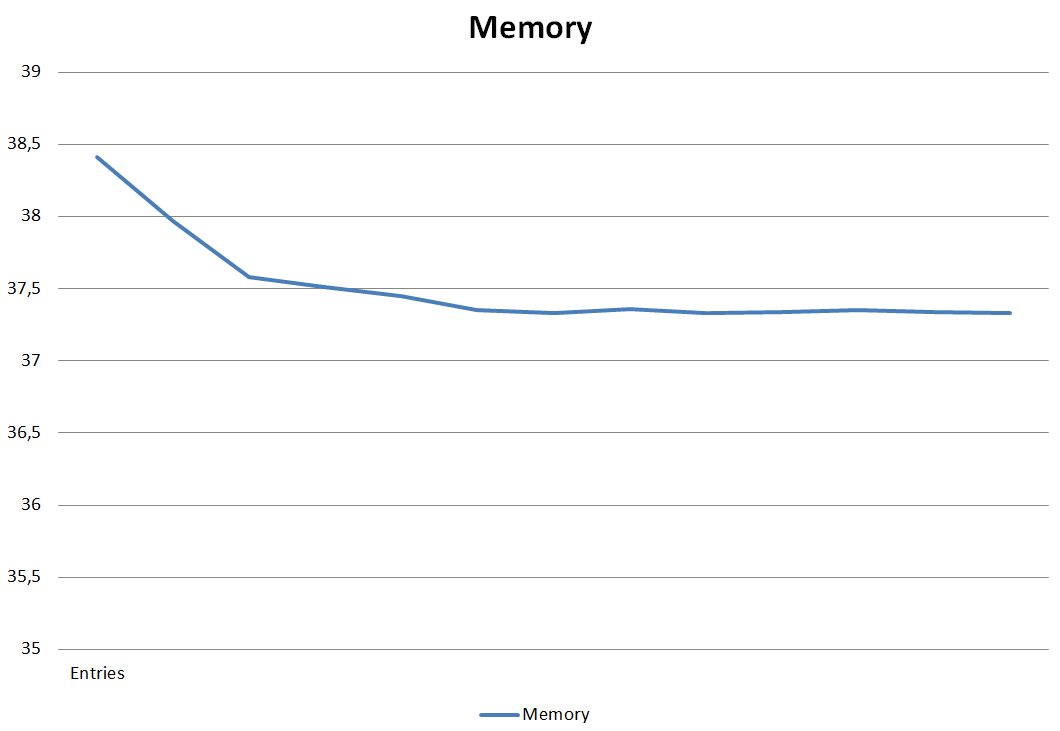
\includegraphics[width=0.82\textwidth]{SkiplistMemory}
      \caption{The average memory usage per entry, plotted against the total number of entries.}
    \end{figure}
\end{frame}

\begin{frame}{Binary search tree}
    \begin{itemize}
        \item For IP adresses: Significantly faster insertions than both other structures for low numbers of entries.
        \item Scales badly compared to the other structures.
        \item Other keys: Always slower than a hash table.
    \end{itemize}
\end{frame}

\begin{frame}{Hash table}
    \begin{itemize}
        \item Significantly higher query speed in all situations compared to other structures.
        \item Faster insert speed as well in most situations.
        \item Highest memory usage in all cases.
    \end{itemize}
\end{frame}

\begin{frame}{Skiplist}
    \begin{itemize}
        \item In no tested situations the fasted structure.
        \item Similar performance to a BST for large numbers of entries.
        \item Always the lowest memory usage, average memory usage goes down with more entries.
    \end{itemize}
\end{frame}

\section{Conclusions}

\begin{frame}{Conclusions}
    \begin{itemize}
        \item Hash table usually the best option.
        \item Binary search tree better for small numbers of simple keys.
        \item Skiplist useful for low memory usage.
    \end{itemize}

    Source code: \url{http://goo.gl/1u1k5I}
\end{frame}

\end{document}
